\section{Demo}\label{Demo} % TODO: crop individual difures

%\def\demofig#1{%
%{\centerline{\includegraphics[width=.95\linewidth, page=#1]{figures/Demo}}}%
% {\centerline{\includegraphics[width=1.02\linewidth, page=#1]{figures/Demo}}}%
%}

FFL is designed to help authors augment formulas with a lightweight syntax and live feedback. Here, we illustrate the envisioned user experience of FFL with a scenario.

% Imagine Auggie, a researcher writing a passage of a \zed{web article in Markdown} where they introduce the idea of linear regression.\footnote{This example is adapted from an excerpt from \cite[Hohman et al.]{ref:hohman2019gamut}.} 

Imagine Auggie, a researcher writing \zed{an article in a web-based scientific authoring environment.} They are writing a passage where they introduce the idea of linear regression.\footnotemark\ They wish to help readers understand the gist of this formula, despite the dense appearance of the formula and the accompanying prose: \footnotetext{This example is adapted from an excerpt from \cite[Hohman et al.]{ref:hohman2019gamut}.}\\

\aptLtoX[graphic=no,type=html]{\centerline{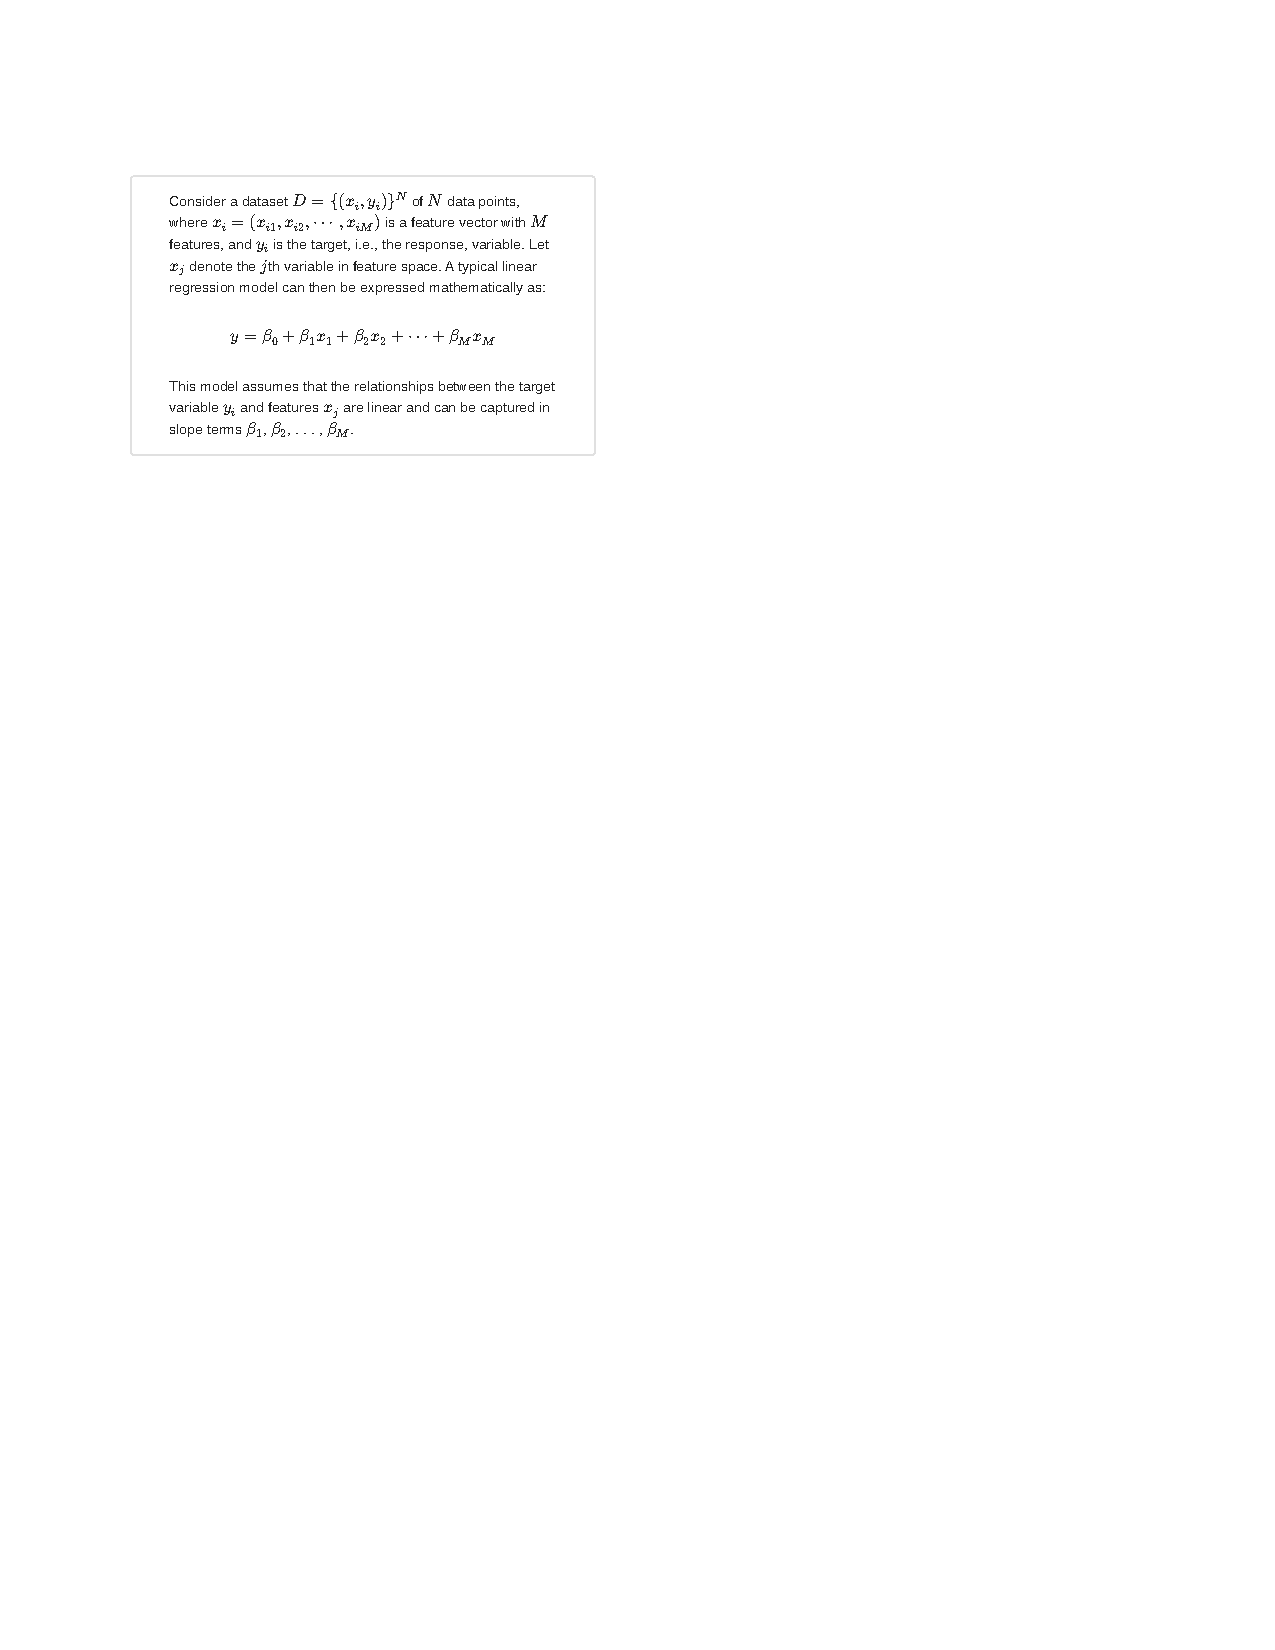
\includegraphics[width=1.02\linewidth]{fig/P4-1.pdf}} }{ \demofig{1}
\Description{An excerpt from a math text that explains a formula for linear regression. The excerpt contains two inline formulas within the text, one block formula, and half a dozen references to individual symbols.} } 


Auggie desires to augment the formula using colors and labels to expose the formula's meaning. Their editor has been extended with support for FFL, which allows them to experiment with these augmentations. Auggie first explores how they could use of color to help readers correlate expressions in the formulas with their descriptions in the text.


To start, Auggie colors the target variable $y$. To do this, they write the following FFL selector and style in a text editor adjacent to their document markup. This helps ensure that the augmentation markup does not clutter the formula or document markup. \\

\aptLtoX[graphic=no,type=html]{\centerline{
\includegraphics[width=1.02\linewidth]{fig/P4-2.pdf}} }{ \demofig{2}\Description{An FFL augmentation specification, consisting of the selector “$y$” and a declaration to color the matching expressions red.}}  

This markup represents a request to find all instances of symbols described by the LaTeX literal ``\$\texttt{y}\$'' and color them red. The effect is instantaneous: as soon as Auggie finishes typing ``\texttt{red},'' the symbol $y$ is colored red everywhere it appears in the document: \\[1ex]
\aptLtoX[graphic=no,type=html]{ \centerline{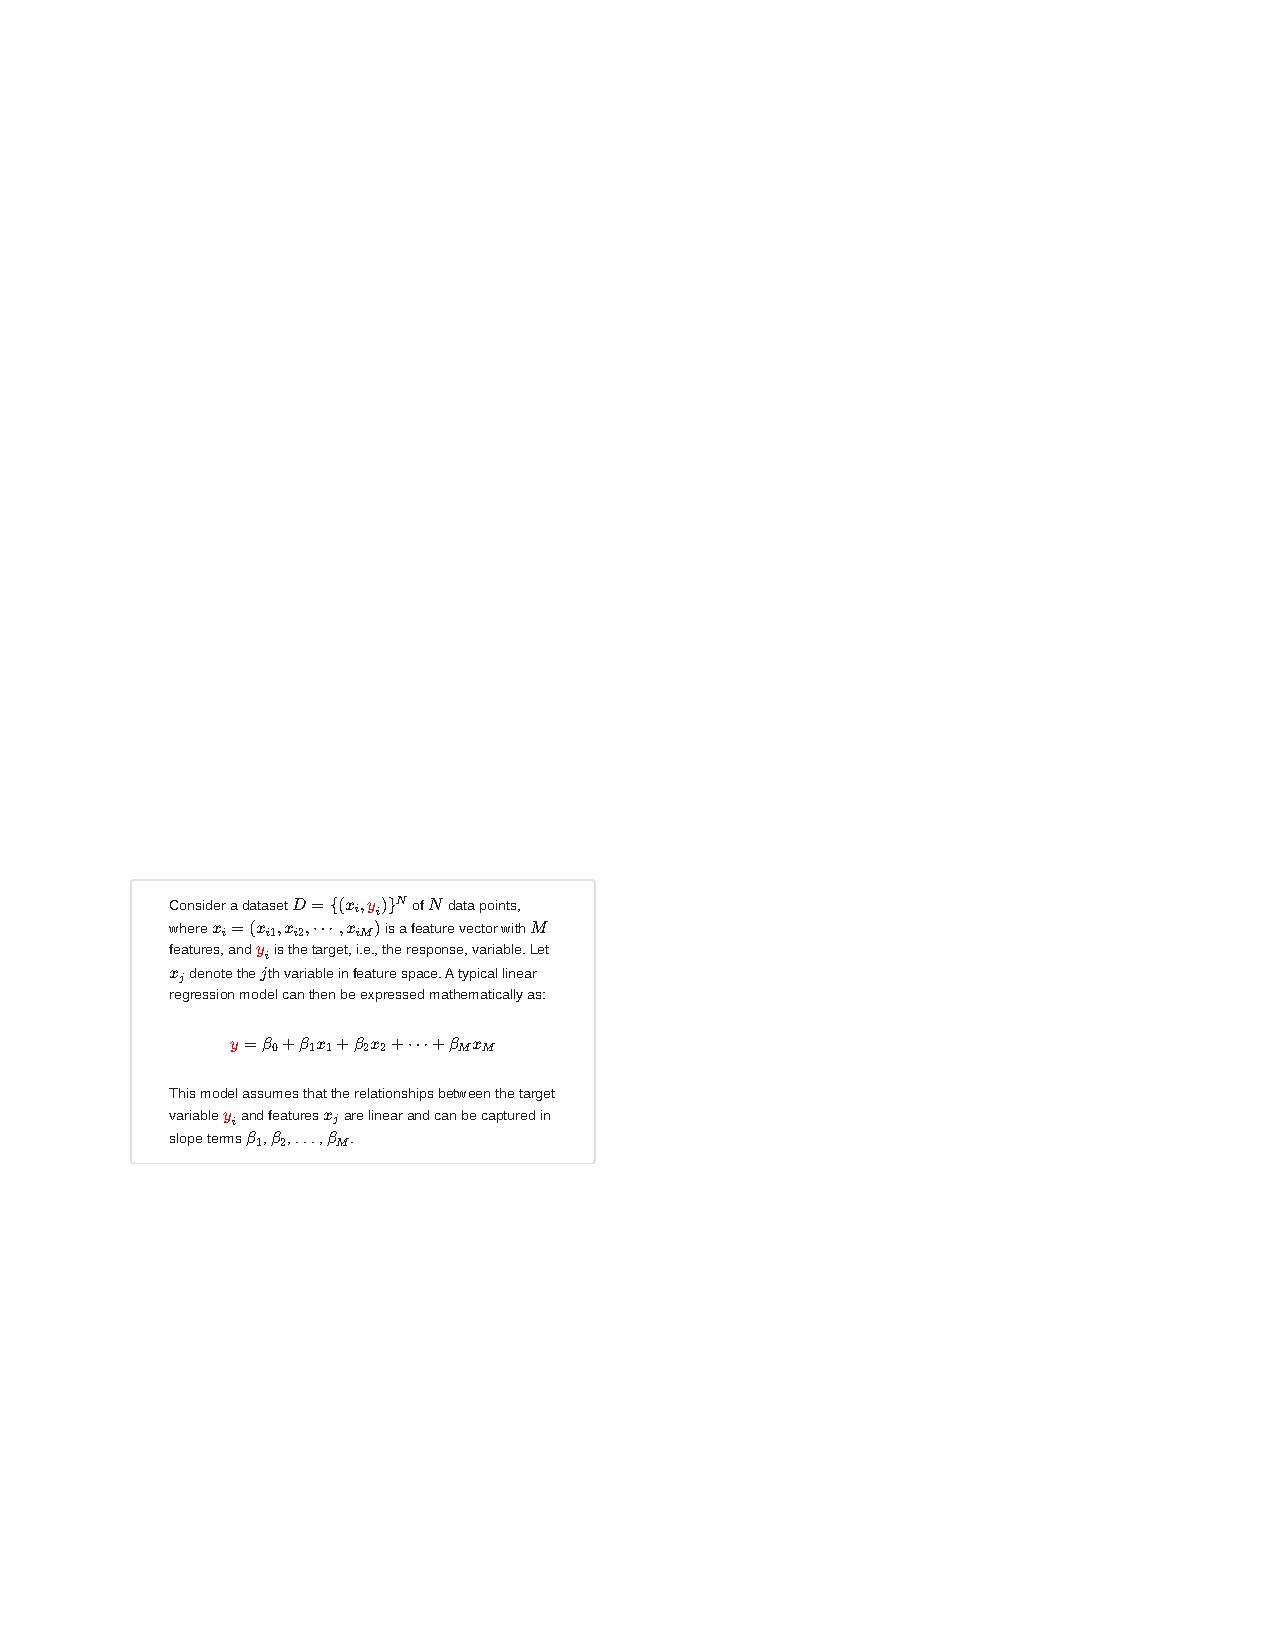
\includegraphics[width=1.02\linewidth]{fig/P4-3.pdf}} }{ \demofig{3}\Description{The excerpt of the math text, augmented to color the variable “y” red wherever it appears in the block formula, inline formulas, and text.} } 

The next step is to use color to help readers find the description of $y$ in the text.
\zed{As Auggie is writing in a web-based environment, they can mix in some CSS to format the text. The CSS can be written alongside the FFL.}

\zed{To style the text,} Auggie surrounds the definition phrase with a \texttt{span} tag and gives it the class ``\texttt{target}.'' Then they give the definition the same color by adding \zed{a selector for the span}, ``\texttt{*.target}'', next to the FFL selector. \\[1ex]
\aptLtoX[graphic=no,type=html]{ \centerline{
\includegraphics[width=1.02\linewidth]{fig/P4-4.pdf}} }{ \demofig{4}\Description{An updated FFL augmentation specification. The selector “star-dot-target” has been added to the list of selectors that will be formatted with the same red color as above.}\\[-1ex] } 

\aptLtoX[graphic=no,type=html]{ \centerline{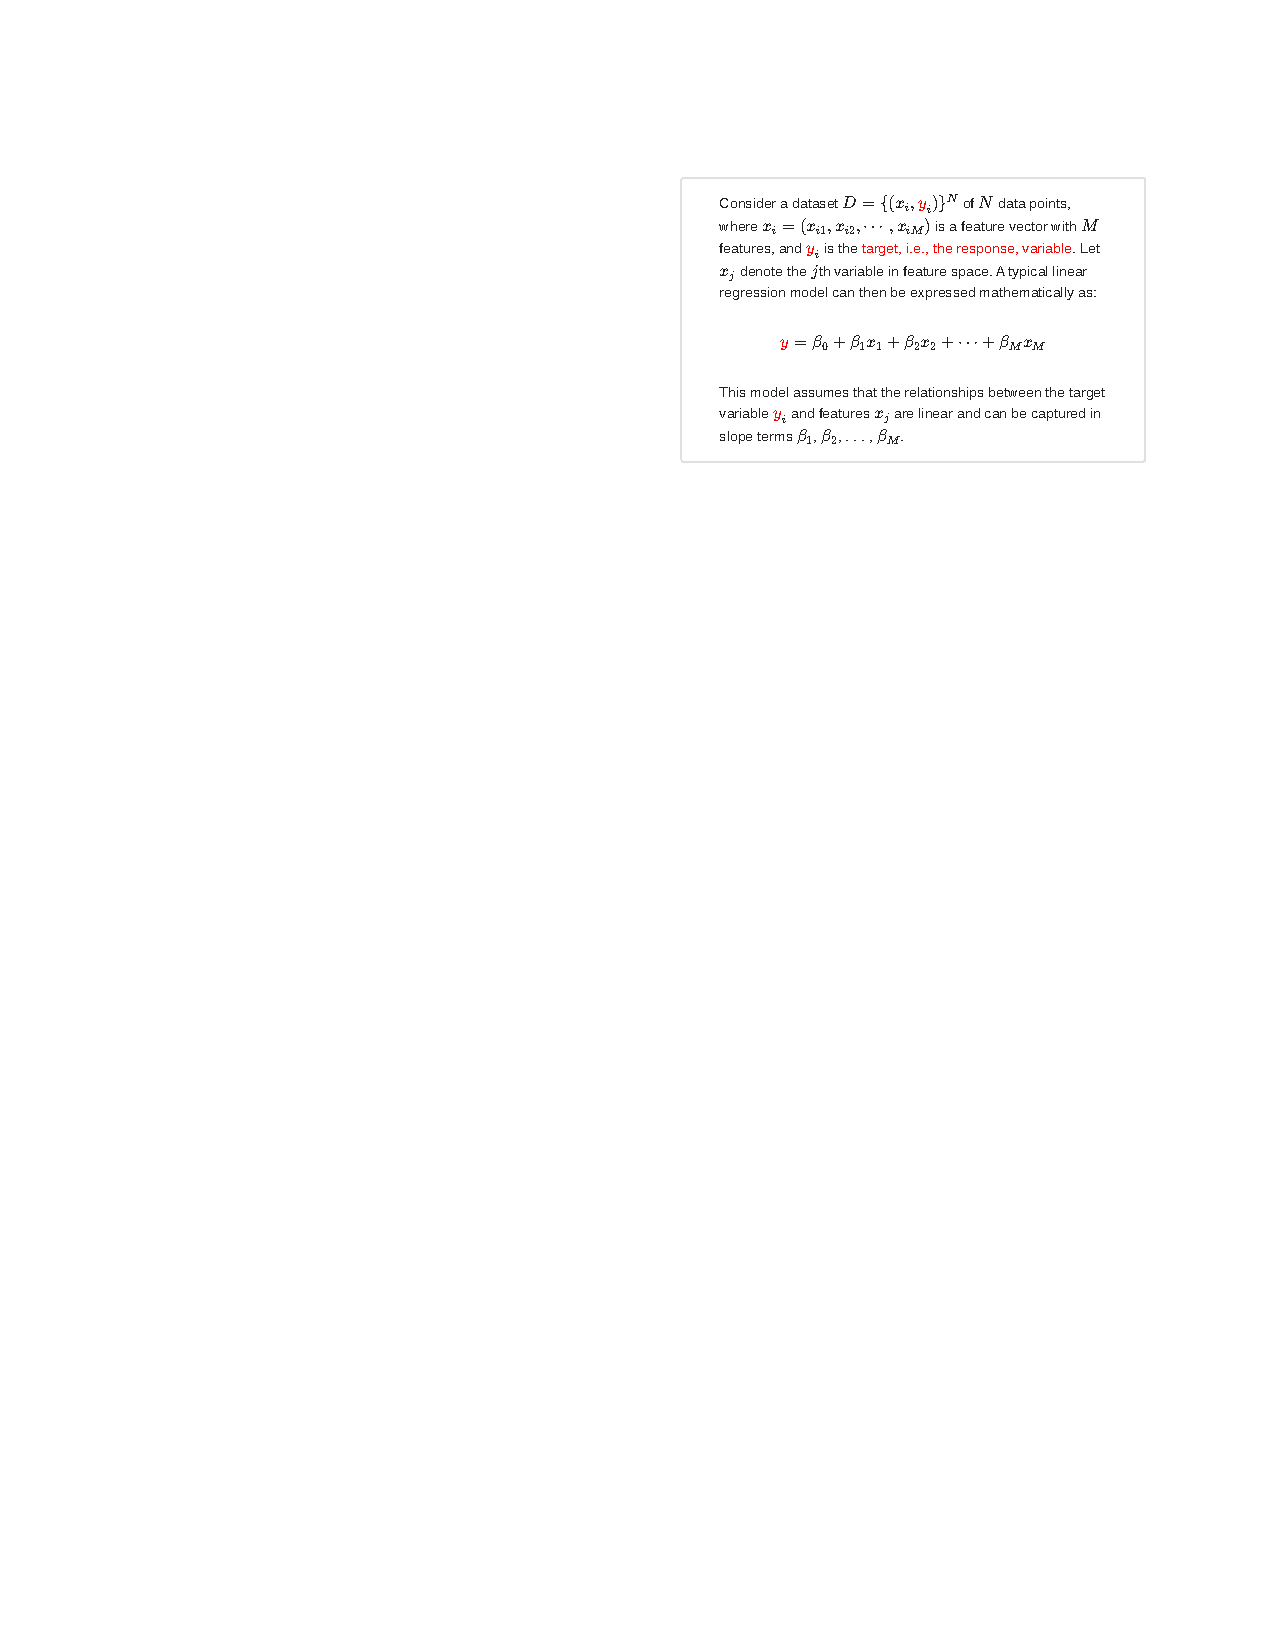
\includegraphics[width=1.02\linewidth]{fig/P4-5.pdf}} }{ \demofig{5}\Description{The excerpt of the math text, with the span of text with the “target” class colored red. This newly-highlighted text reads “target, i.e., the response, variable.”} } 


Auggie is not content with the augmentation, wishing to try out other, less harsh colors. As they experiment with other colors from \texttt{DarkRed} to \texttt{Crimson}, they see the visual effect live, 
receiving the rapid feedback common to online Markdown editors, but less common to LaTeX document editors that require recompilation. \\[-1ex]

\aptLtoX[graphic=no,type=html]{ \centerline{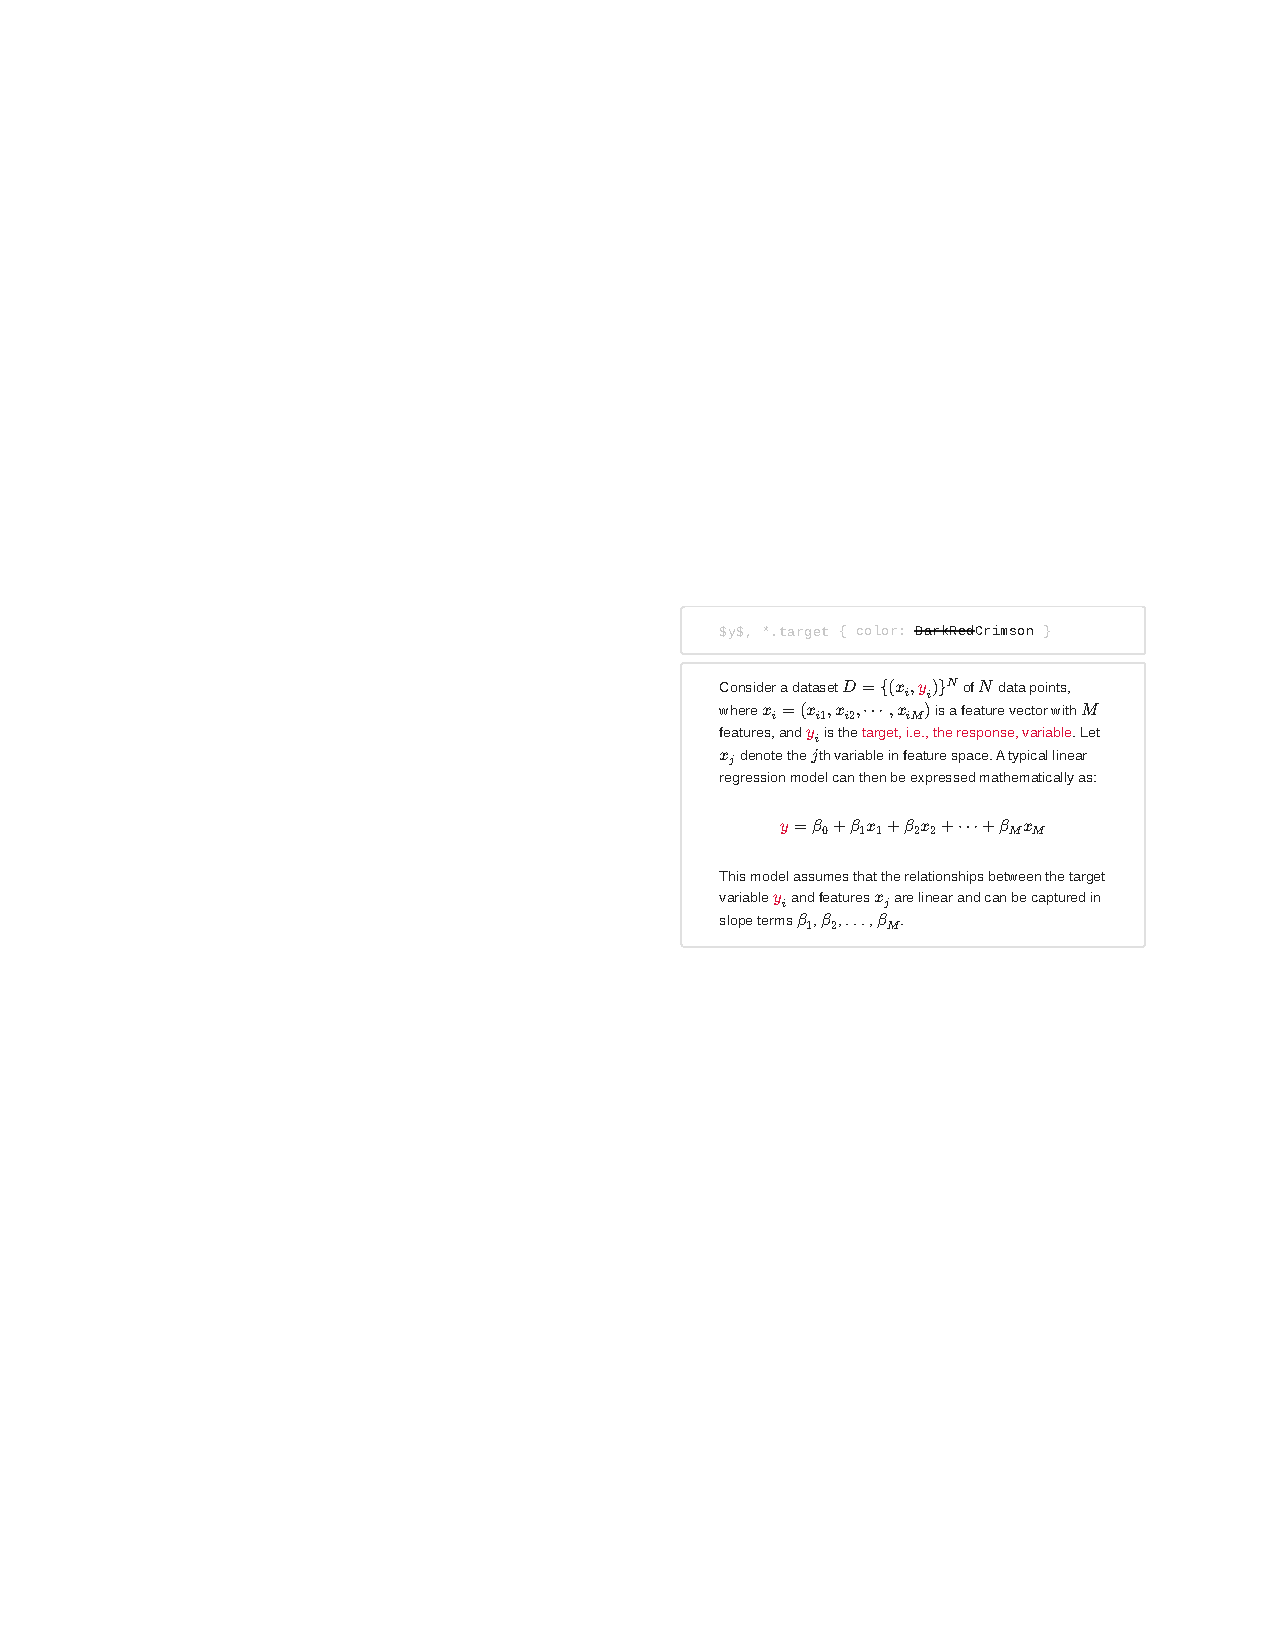
\includegraphics[width=1.02\linewidth]{fig/P4-6.pdf}} }{ \demofig{6}\Description{An updated FFL augmentation specification. The color property has been changed first to DarkRed, and then to Crimson.}
\demofig{7}\Description{The excerpt of the math text, where the text that was colored red before is now colored crimson.} } 


Now that Auggie is content with the colors they chose, they notice that they wish for the subscripts of $y$ expressions to be colored as well. To augment all $y$ expressions with subscripts, Auggie only needs to make a small edit.
They add ``\texttt{\$y\_*\$}'' to the list of selectors, and see the crimson color applied to the intended expressions. \\ 

\aptLtoX[graphic=no,type=html]{ \centerline{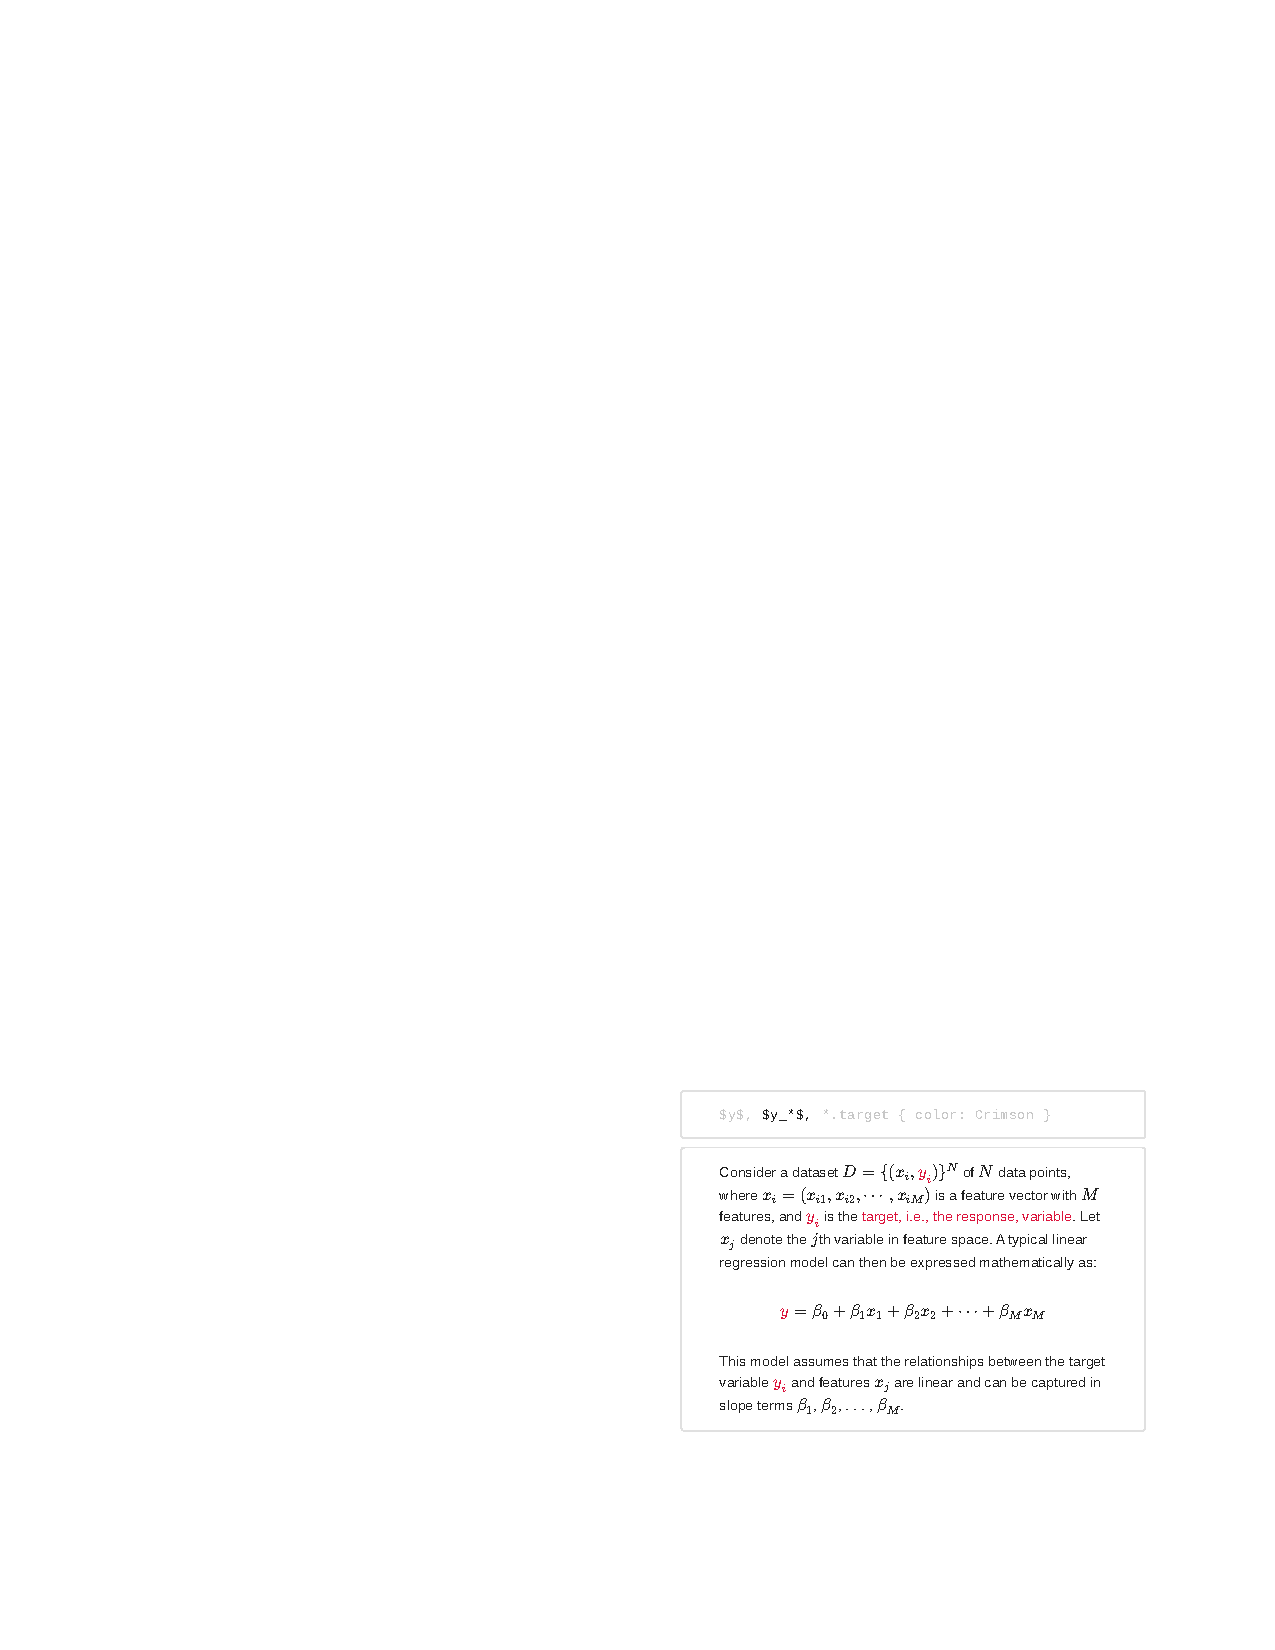
\includegraphics[width=1.02\linewidth]{fig/P4-7.pdf}} }{ \demofig{8}\Description{An updated FFL augmentation specification. The selector “dollar-sign-y-underscore-start-dollar-sign” has been added to the list of selectors that will be formatted with crimson color.}
\demofig{9}\Description{The excerpt of the math text, with all symbols consisting of “y” and a subscript are now colored crimson as well.} } 


The next step is to help readers understand the other major expressions in the formula, namely the $x$'s (\textcolor[HTML]{005A9C}{{blue}}) and $\beta$'s (\textcolor[HTML]{9370DB}{{purple}}). Auggie decides to assign each a distinct color that will help a reader look up the respective definitions in the text. To do so, they create a similar style block for each group of variables they wish to augment:\\[1ex]
\aptLtoX[graphic=no,type=html]{ \centerline{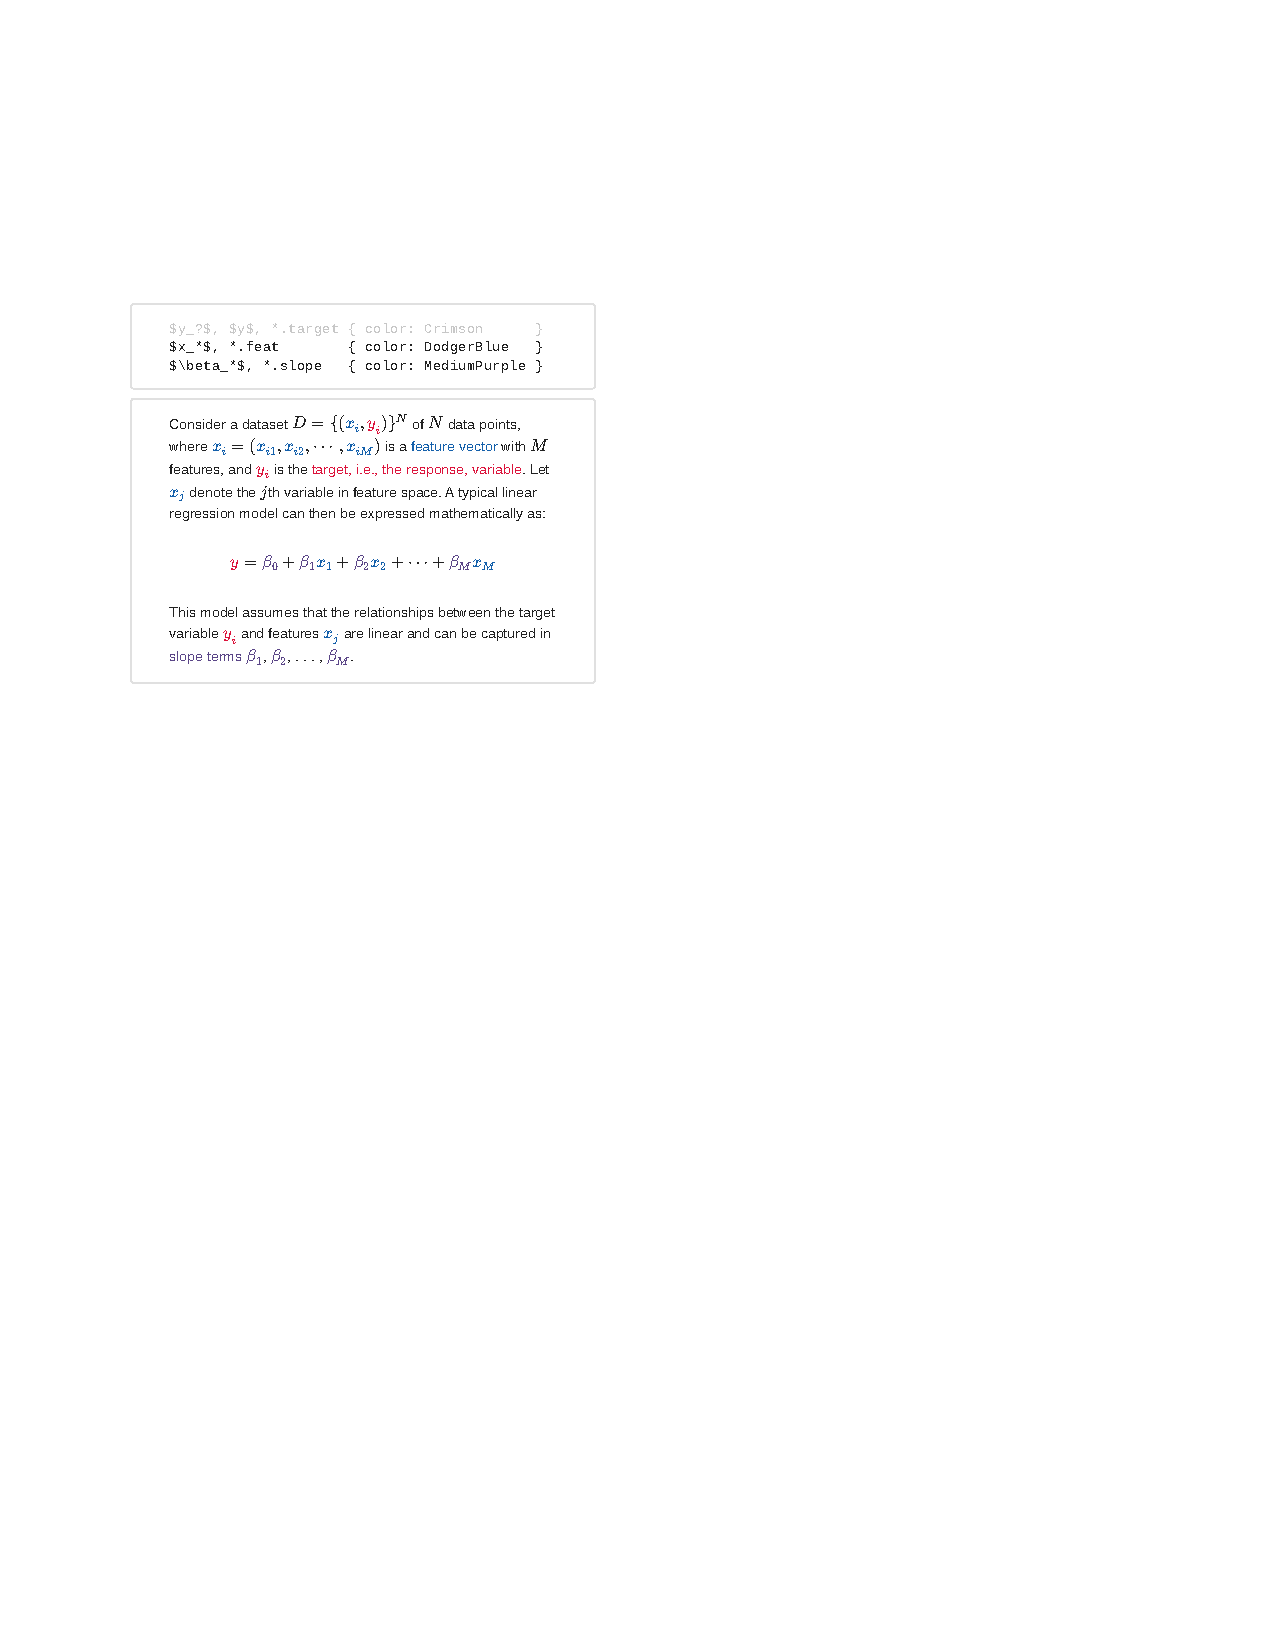
\includegraphics[width=1.02\linewidth]{fig/P5-1.pdf}} }{ \demofig{10}\Description{An updated FFL augmentation specification. Two new augmentation rules have been added. The first rule consists of a selector for “dollar-sign-s-underscore-star-dollar-sign” and “star-dot-feat”, and a property to color matching expressions “DodgerBlue”; and a selector for “dollar-sign-beta-underscore-star-dollar-sign” and “star-dot-slope,” and a property to matching expressions MediumPurple.}\\[-1ex]
\demofig{11}\Description{The excerpt of the math text, with a few changes. All symbols related to “x,” and the phrase “feature vector” are colored with the color “DodgerBlue.” All symbols related to “beta” and the phrase “slope terms” are colored with the color “MediumPurple.”} } 


After inspecting the augmented passage, Auggie wishes that $\beta_0$ was not given the same color as the other $\beta$ terms, because it is better described as an intercept rather than a slope term. They revert the style for just $\beta_0$ by adding an additional one-line rule, setting the color of $\beta_0$ to \texttt{inherit}, as one might do in CSS, rather than accept the color of the other $\beta$ terms.\\

\aptLtoX[graphic=no,type=html]{ \centerline{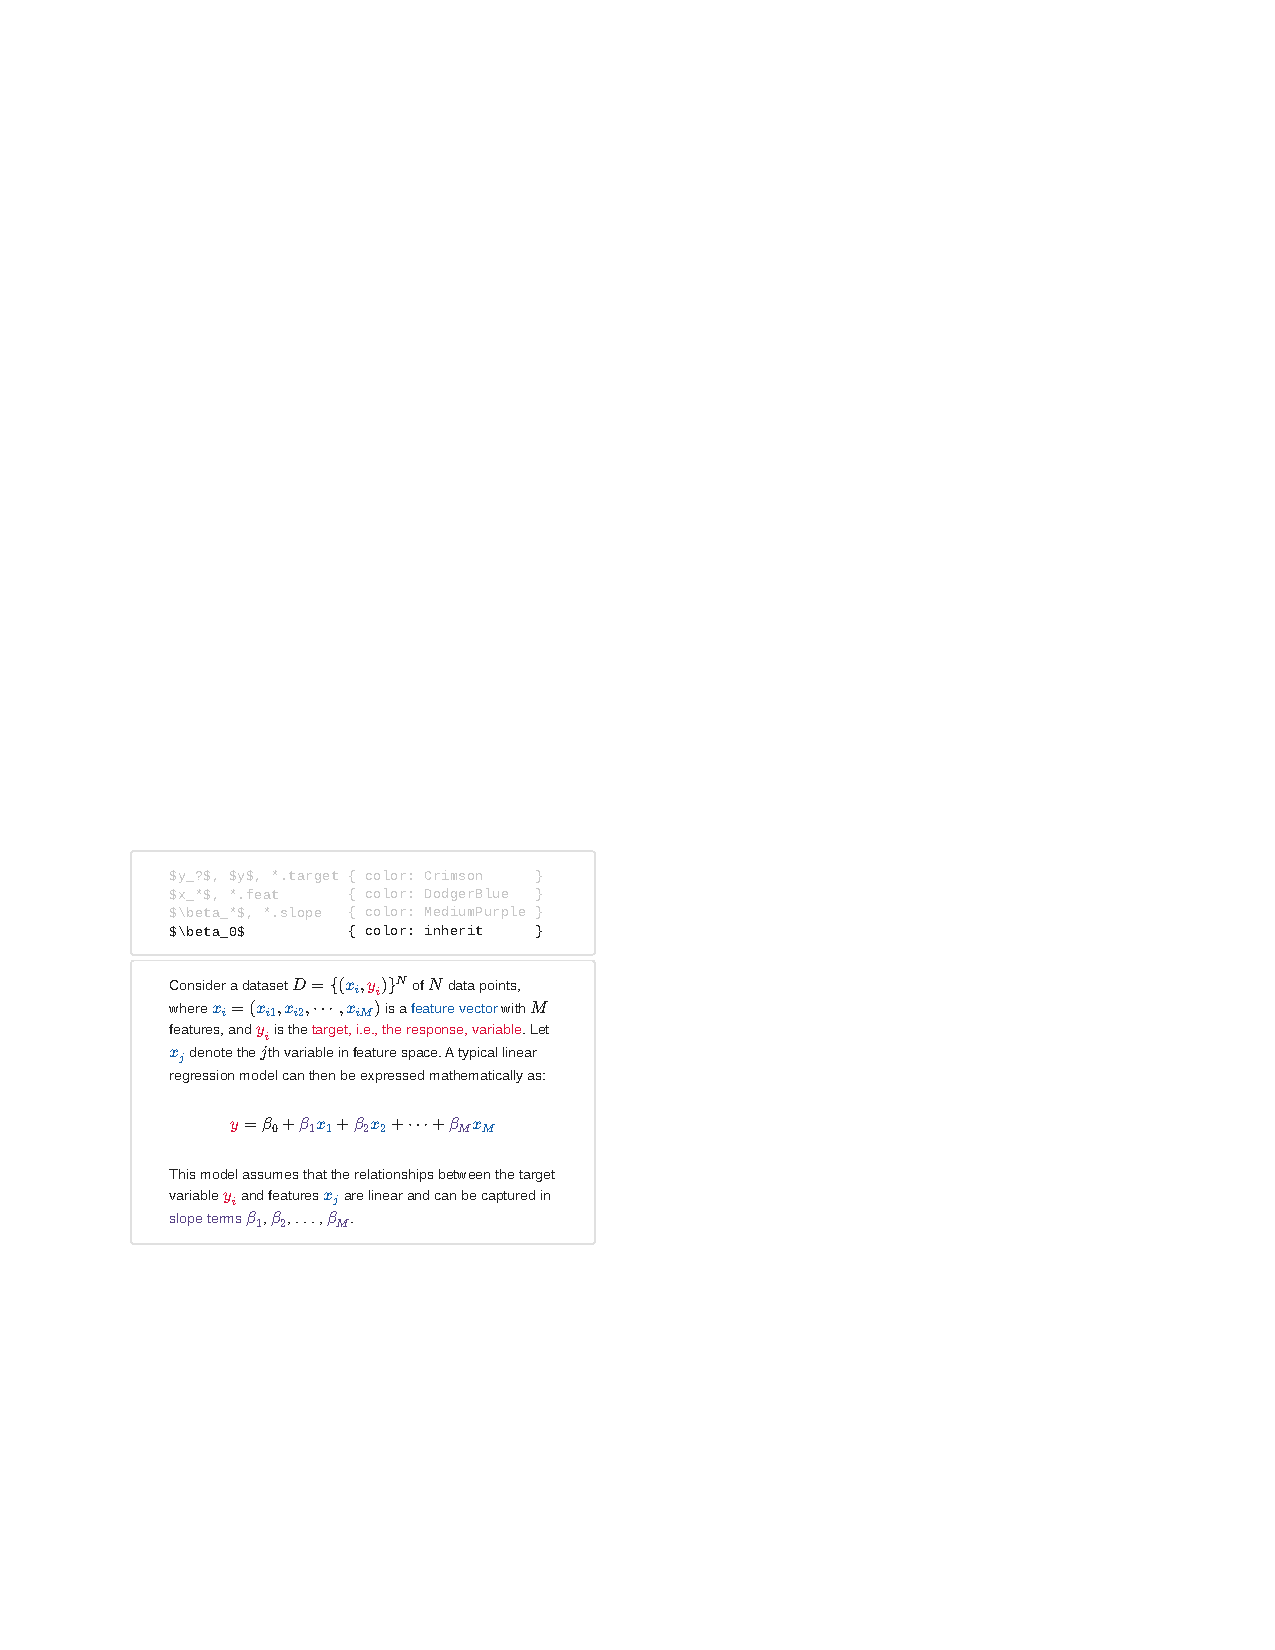
\includegraphics[width=1.02\linewidth]{fig/P5-2.pdf}} }{ \demofig{12}\Description{An updated FFL augmentation specification. One new augmentation rule has been added. The selector is “dollar-sign-beta-subscript-zero-dollar-sign,” and the accompanying style property is “color” with the value “inherit.”}\demofig{13}\Description{The excerpt of the math text, this time with “beta-sub-0” colored black instead of purple.} } 


Auggie is satisfied with this result. Throughout their exploration, FFL provided a lightweight syntax for making cross-cutting notation augmentations with live feedback.
% And after only a few simple steps like these, now readers can navigate back to relevant elements in the text just with the colors.

\subsubsection*{Further design space exploration} There is more than one way to augment a formula to expose its meaning. Auggie considers another strategy that they think will make their article more skimmable which relies less on the textual description (omitted below), and instead exposes descriptions of expressions in labels. FFL helps them experiment with this style of augmentation as well.

Auggie starts from a fresh FFL style sheet, this time adding augmentations in the form of labels. They first add a label for $y$, describing it as the ``target'' of prediction.\\[1ex]
\aptLtoX[graphic=no,type=html]{ \centerline{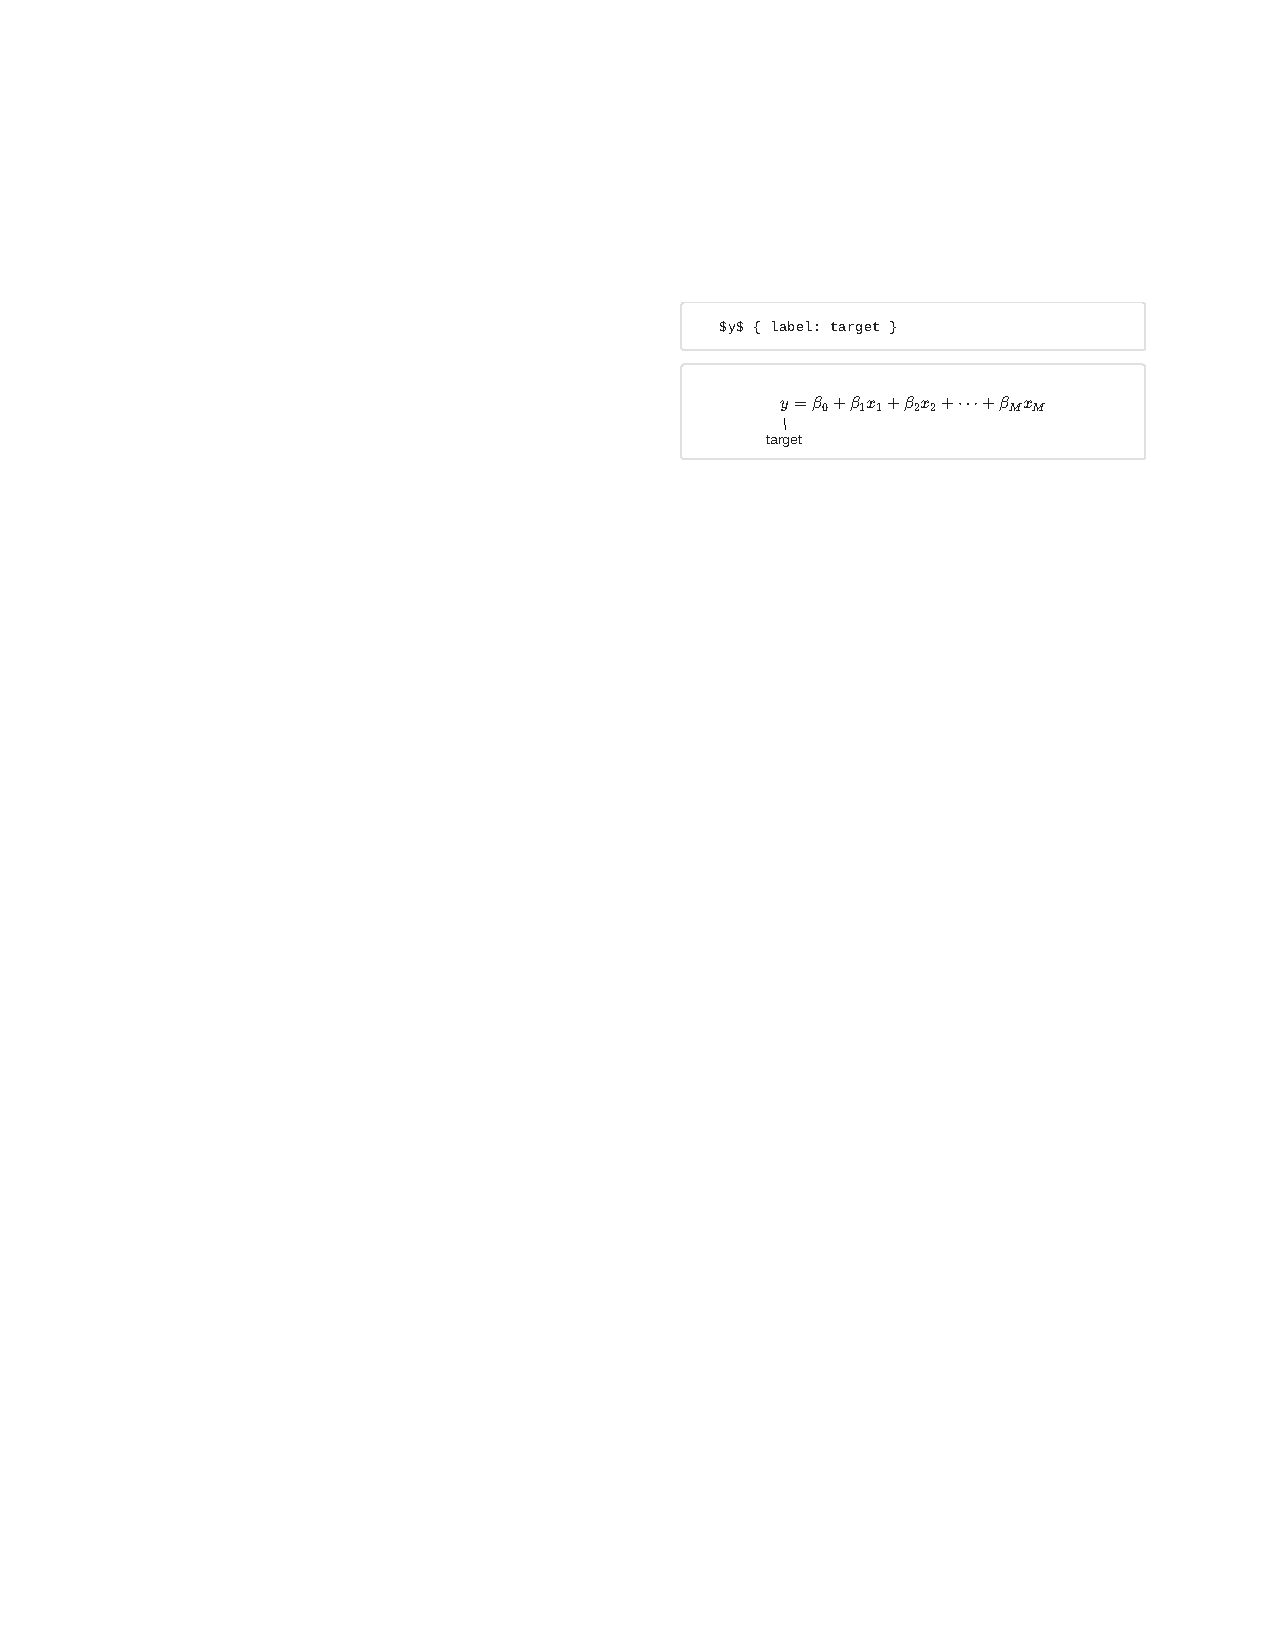
\includegraphics[width=1.02\linewidth]{fig/P5-3.pdf}} }{ \demofig{14}\Description{A new FFL augmentation specification, with the selector “dollar-sign-y-dollar-sign,” and the property “label” with the value “target.”}\\[0ex]
\demofig{15}\Description{The linear regression formula with “y” labeled with the word “target.”} } 


They then add labels for the remaining expressions. This is a matter of adding one style block per annotated expression.

\aptLtoX[graphic=no,type=html]{ \centerline{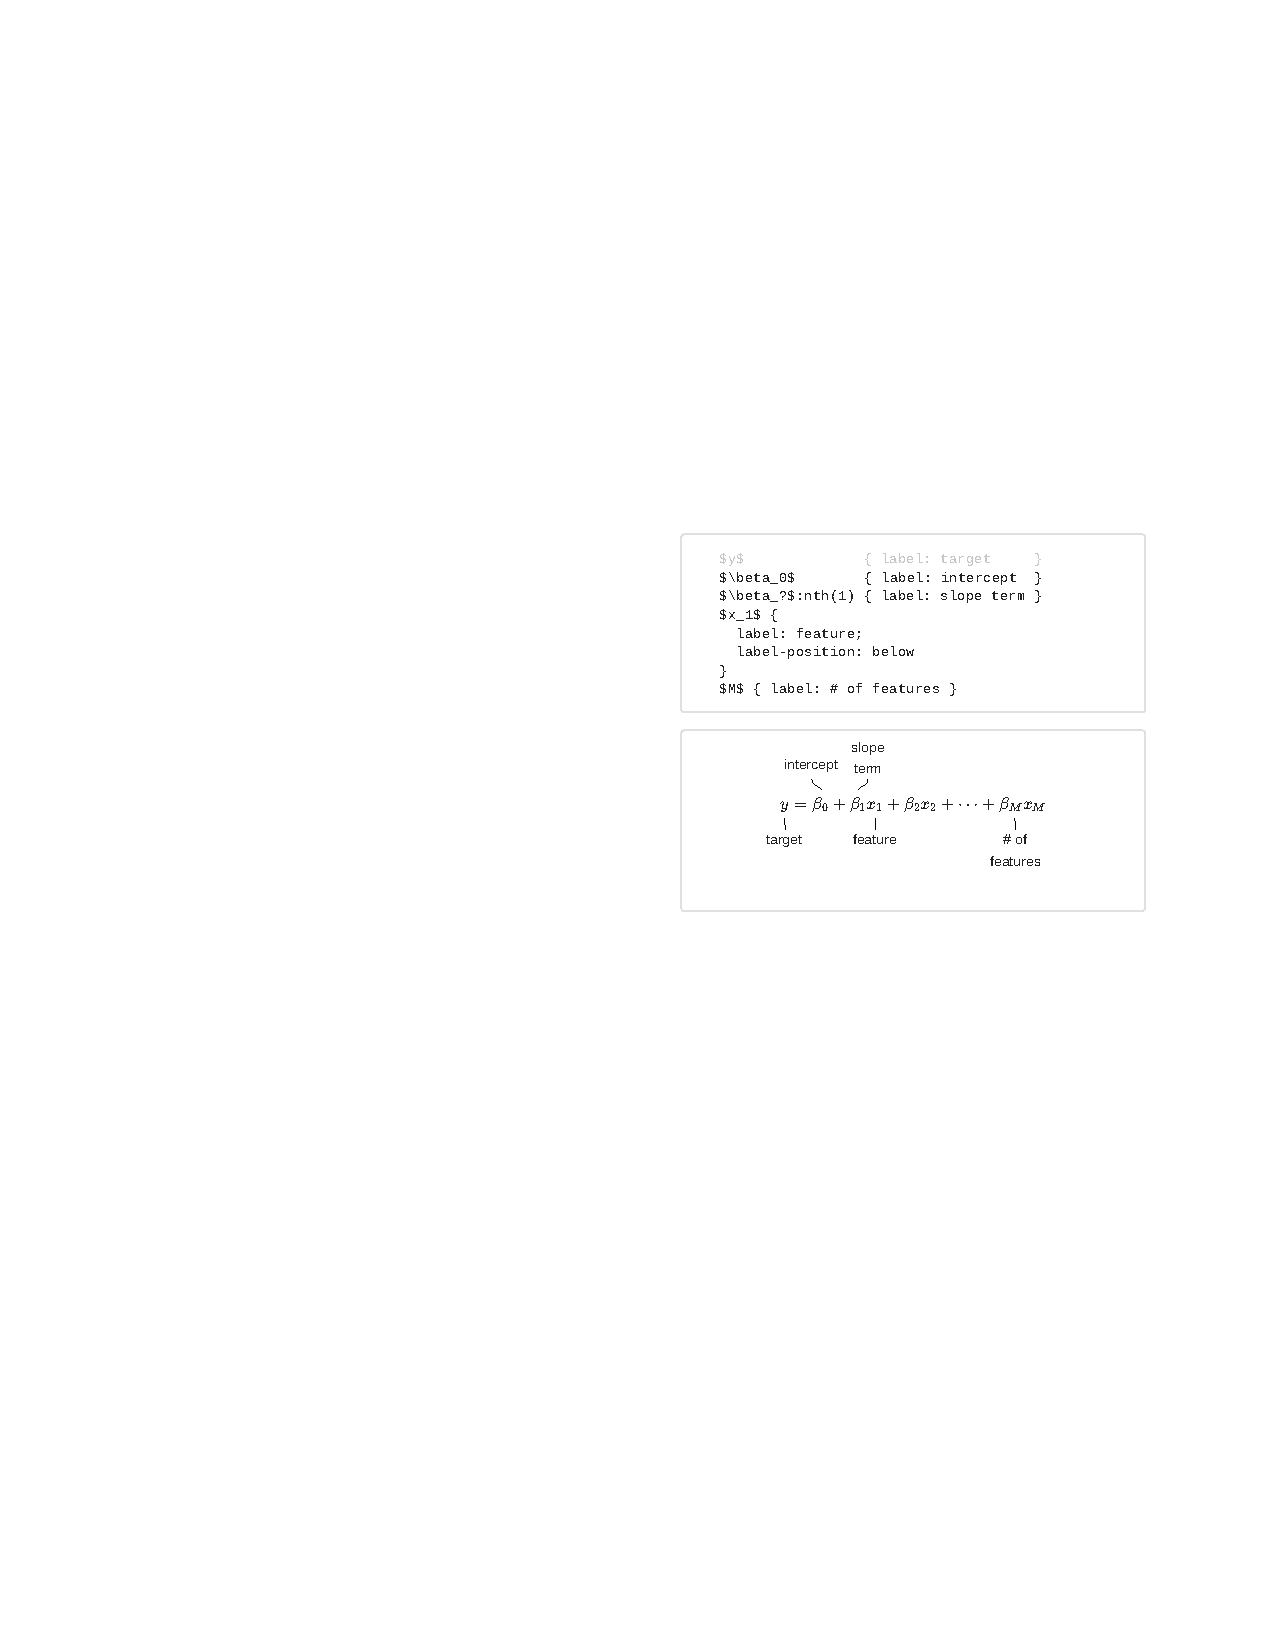
\includegraphics[width=1.02\linewidth]{fig/P5-4.pdf}} }{ \demofig{16}\Description{An updated FFL augmentation specification, extended with rules for adding labels for 4 additional expressions. Each rule consists of the label property and a value of what the label should read. One of the selectors uses the “label-position” property to specify the label should appear “below” the formula.}
\demofig{17}\Description{The linear regression formula with labels as follows: “y” is labeled “target”; “beta-sub-0” is labeled “intercept”; “beta-sub-1” is labeled “slope term”; “x-sub-1” is labeled “feature” and the label appears below the expresion; “beta-sub-M” is labeled “number of features.”} } 


As Auggie does so, labels render live. The labels are automatically laid out to reduce overlap and maximize adjacency of labels to expressions. In this way, Auggie can think about augmentations at a high level, avoiding the work of manually arranging  labels. Notably the labels are tolerant to future changes to the formula: should Auggie add additional $\beta$ and $x$ terms to the formula, the labels will move as the formula adjusts its position. 
% And this above is all they need to write. No more low-level ``drawing'' commands because it is just \texttt{label} in FFL; No more meticulously shifting labels around to make space for new ones because FFL spaces them automatically; And again, there is no need to wait for compilation to confirm that their positions are as intended. \\

When they are finished with this document, Auggie could save their style sheet for use in other documents with notation that deserved to be described in similar ways.
%in another document with related or similar content, or even use different style sheets for the same document in different situations, all achieved through using FFL.

% We explain the experience of interacting with FFL by describing a scenario in which an envisioned author experiments with styling a formula. We walk through the process of augmenting the formula from Hohman et al.'s \emph{Gamut} project \cite{Gamut}. \andrew{Can we pick another example that is not from Fred's work? Perhaps we can pick an example that was from the web.}

% \andrew{The key examples that I want to show in a demonstration of the tool are:}

% The payoff of using FFL arises when there are many augmentations at once, and they apply across a larger document.

% Points at which to show improvement:

% 1. Cleanliness of markup
% 2. Simplicity of basic literal matching
% 3. Ability to apply styles across a formula (including using wildcards)
% 4. Support for good default label styling

% \andrew{One motivation of the toolkit as it is currently designed is that an author should be able to write a selector just as easily if they are looking at the rendered form or at the underlying markup. Some tolerance to variation in markup is therefore programmed into the runtime environment (though in the limitations section we describe where our current technical approach falls short).}

\section{System}

In the section, we describe FFL, a language and live runtime for augmenting typeset math formulas in web documents. FFL was designed and developed following an iterative approach. Fine-grained decisions about syntax design were informed by pilot usability studies with early versions of the tool.

Acknowledging the challenges of writing augmentation markup revealed in prior work~\cite{ref:head2022math}, the goals of FFL were as follows:

% We now describe FFL, a language for augmenting math formulas. In designing FFL, we adopted an iterative approach, conducting informal formative interviews and pilot studies of prototype highlighting tools. These iterations helped us make decisions around fine-grained aspects of FFL's syntax, such as what wildcards should look like, and what syntax should be used for selecting fragments of formulas. Our main design objectives revolve around several key concerns raised in \cite[Head et al.]{ref:head2022math} and aim to address the following,

\begin{itemize}
\item Basic augmentations should be easy to read and write;
\item Authors should receive rapid feedback on their designs;
\item Augmentations should be aesthetically pleasing;
\item Authors should be supported to experiment with cross-cutting augmentation choices.
% \item \textit{Interactivity}: Our tool should allow dynamic representation of formula;
% \item \textit{Ease of Use}: Basic styling should be easy to both implement and understand;
% \item \textit{Pretty Defaults}: It should not require a massive amount of tweaking to achieve usable results; and
% \item \textit{Reusability}: Configurations should be able to be reused to make cross-cutting or repeated styling elements.
\end{itemize}

Below, we describe the two main components of the FFL toolkit: the language, and the supporting live runtime.

% FFL comprises the following main components:
% \begin{enumerate}
%     \item A language similar to CSS for selecting and augmenting math expressions;
%     \item A runtime that supports the live application of styles to formulas that are typeset using the popular KaTeX web formula renderer.
% \end{enumerate}

\subsection{Language design}

% \andrew{It feels important for us to note in the text that we don't think that the current specification of FFL is complete, but rather a starting point for a more comprehensive set of augmentations. The main parts of the language---of selectors, styles, and annotations---is our major contribution, as well as the development of what we think are going to be the most powerful, general-purpose features.}

\begin{figure*}
    \centering
    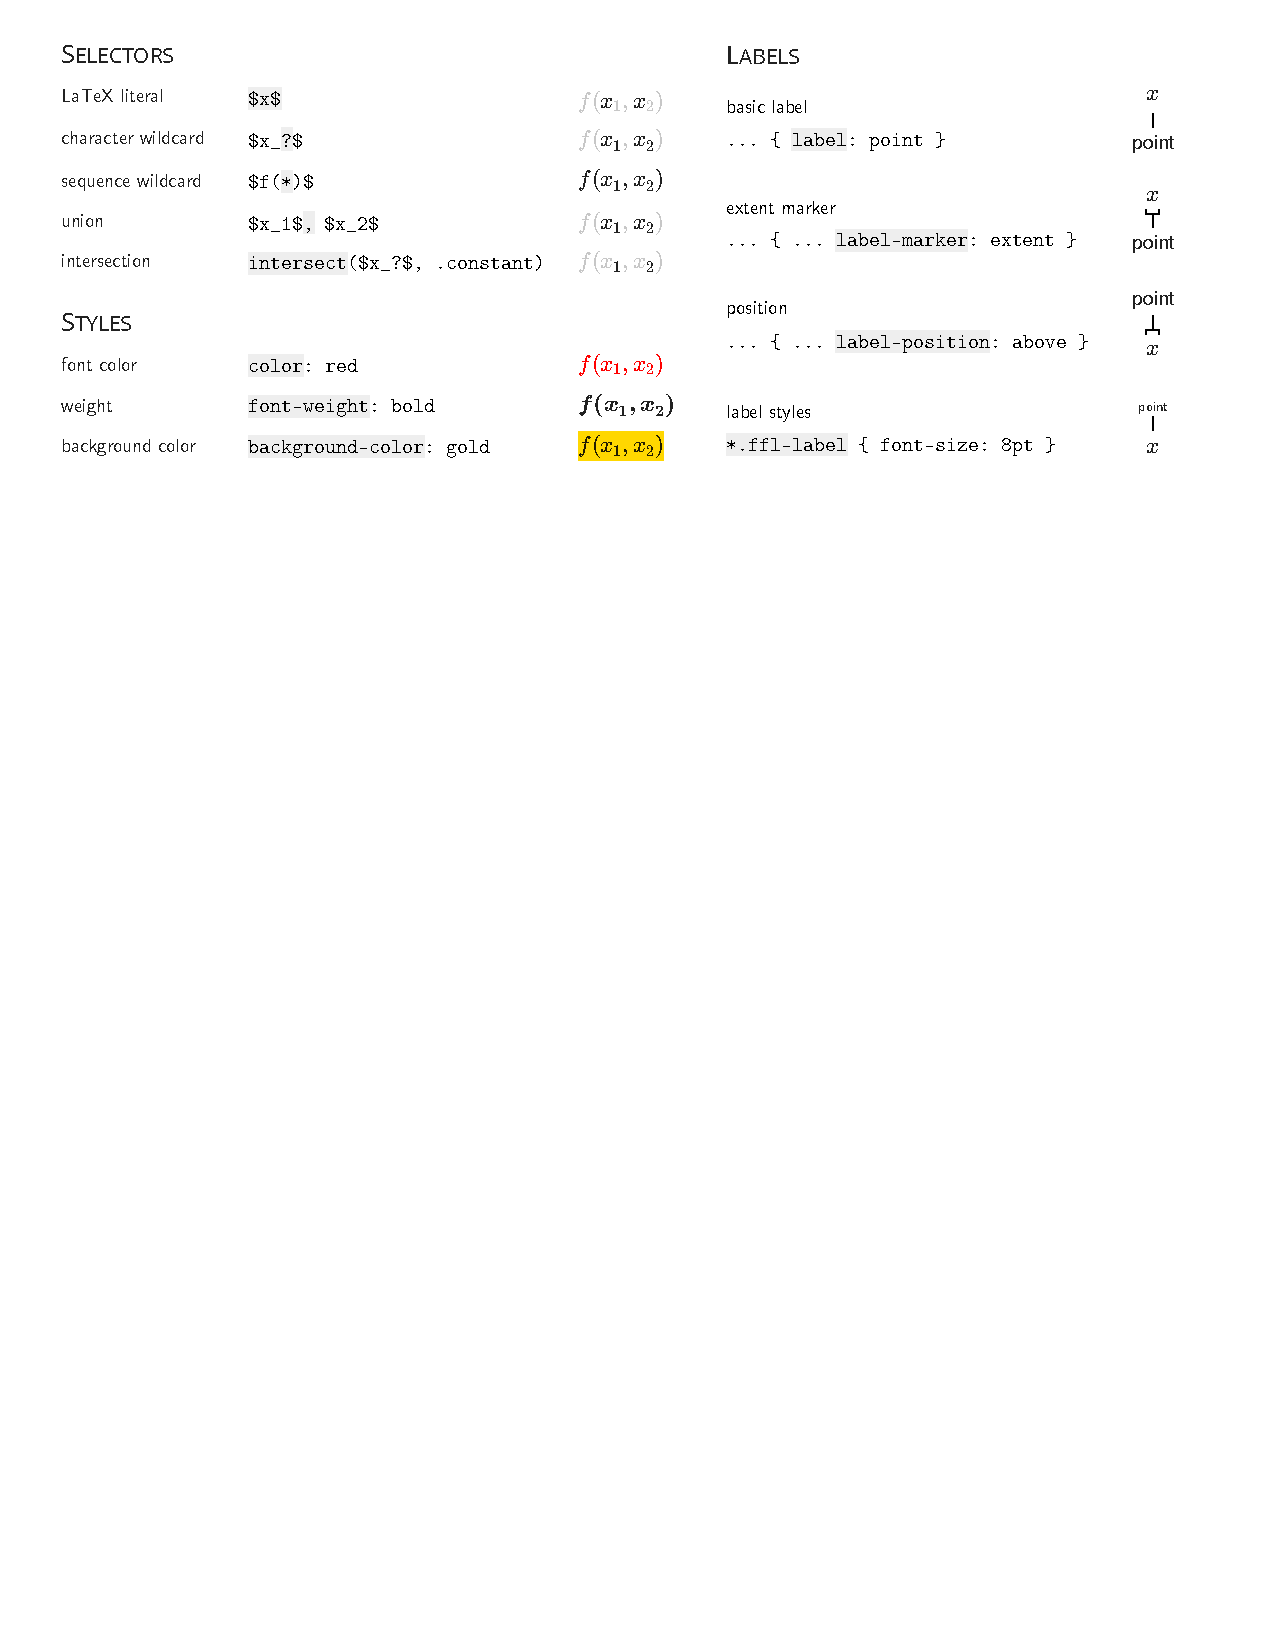
\includegraphics[width=.95\linewidth]{figures/Language}
    \caption{A visual specification of the FFL language, including its constructs for selecting expressions, styling, and labeling formulas. \normalfont Each row names a language feature, provides an example snippet of FFL, and shows the result of its application to one of the example formulas $f(x_1, x_2)$ or $x$.}
    \Description{A table showing features of the FFL language. In each row is the name of the feature, an example of an FFL spec using that language features, and a render of a formula that has been augmented with that spec. Features include: for selectors: literal selectors, character and sequence wildcards, union, and intersections. For styles: font color, weight, and background color. For labels: simple labels, extent markers, label positions, and additional styles.}
    \label{fig:language_examples}
\end{figure*}

% \andrew{Figures: @Zed, what is your current thinking around having a BNF declaration of the language?} probably more formal than we need to be since we already have the feature figure

The FFL language is a CSS-like language for specifying augmentations for formulas. FFL was designed to resemble CSS due to the latter's use as a separable styling language in web authoring environments. We envisioned authoring environments where eventually authors write FFL and CSS side-by-side.

\begin{wrapfigure}[5]{l}{0.25\columnwidth}
\vspace{-2ex} % TODO: fix to fit any new position
\begin{Verbatim}[commandchars=\\\{\}]
 \textcolor{darkblue}{$x_i$}, \ldots \{
   \textcolor{magenta}{ color: red; }
   \textcolor{magenta}\ldots
 \}
\end{Verbatim}
\end{wrapfigure}
Like CSS, FFL in essence consists of declarations of style rules. Each style rule block consists of a \textcolor{darkblue}{selector} indicating what expressions the augmentation applies to, and a set of \textcolor{magenta}{property declarations} describing augmentations to apply, resembling the inset figure.

% Primarily, we design the language to resemble CSS, not only in that it is written separately from the document itself for both ease of organization and reusability, but it is also composed of a list of ``style rule'' sets, which in turn are a combinations of \textcolor{blue}{selectors}
% and \textcolor{red}{property declarations}, that are global across a single invocation of our rendering API. A single style rule block generally looks like the following,

One advantage of this format is that FFL can be easily transpiled to CSS for a myriad of simple styles (e.g., color, font weight). Below demonstrates the current expressive potential of FFL's syntax. A visual summary of language constructs appears in Figure~\ref{fig:language_examples}. Our focus is on describing the language primitives, and the augmentations we have built into the language to date. We intend the language to be further extended to support additional augmentations.

% affording us many style properties with a minimal amount of additional implementation. Below is a list of our major contributions, namely selectors and some style properties for both simple styles and additional label annotations (Figure \ref{fig:language_examples}). This by no means indicates that FFL is a complete and closed system, but rather it is meant as a select sample of features which we have so far implemented, in a direction of design that can be generalized and expanded upon, though we do believe that it already covers a fairly common range of use cases.

\subsubsection{Selections}
An author conveys which math expressions to augment by writing \emph{selectors}. FFL provides a flexible selector syntax, allowing for literal matches to LaTeX substrings, wildcards, predefined classes, and combinators.

% While it is relatively painless to apply styles, many of our affordances in fact do still rely on the ability to \textit{select} the desired elements said styles should apply to. 

% We mainly offer two types of selectors, \textit{literal selectors} and \textit{pre-defined classes}.

\paragraph{Literal Selectors} The simplest way to select an expression is to write the LaTeX for the expression one wishes to augment. Writing a literal selector entails writing a LaTeX string, with its typical (\texttt\$) delimiters on either side. Literal selectors are resilient to some simple variations in how an expression might be written in LaTeX: for instance, the selector ``\texttt{\$x\_i\$}'' matches the expression $x_i$ regardless of whether it is written ``\texttt{\$x\_i\$}'' and ``\texttt{\$x\_\{i\}\$}''.

% \paragraph{Literal Selectors}The simplest way to select some elements in formulas is to directly quote the portion of math expression in a pair of dollar signs (\texttt\$), a common delimiter of math mode in LaTeX after which our styles primarily apply to. This also simplifies parsing as it is one of the only characters that cannot be retained inside LaTeX math. Enclosed in the delimiters has no difference from the set of LaTeX math that \textit{KaTeX} supports, except for \textit{wildcards}.

\paragraph{Wildcards} Authors can select syntactically related expressions using wildcards. Two kinds of wildcards are provided, inspired by the \texttt{glob}~\cite{UnixMan} wildcard syntax used in Unix command lines. \emph{Character wildcards} match single characters, and are written ``\texttt{?}''. For instance, ``\texttt{\$x\_?\$}'' selects all symbols that have $x$ as a base and a single character as subscripts. \emph{Sequence wildcards} match strings of unbounded length, and are written ``\texttt{*}''. For instance, ``\texttt{\$f(*)\$}'' selects $f()$, $f(0)$, $f(x)$, and $f(x + 1)$, among other expressions. \zed{Authors can match the literal characters ``\texttt{?}'' and ``\texttt{*}'' by escaping them with a backslash (i.e., as ``\texttt{\textbackslash?}'' and ``\texttt{\textbackslash*}'').}

% \paragraph{Wildcards} Within  a literal selector, any single token can be replaced by a question mark (\texttt{?}) and an any-length sequence a asterisk (\texttt{*}), bounded by groups (\texttt{\{}\dots\texttt{\}}). This is chosen to mirror \texttt{glob}\cite{UnixMan}, which allows for in many cases, the selection of similar segments as well as long ones with a single shortened selector, rather than copying the entire segment one wishes to apply styles to. For example, \texttt{\$m\_?\$} can match $m_0$ or $m_i$ but not $m_{i,j}$ , and \texttt{\$f(*)\$} can match $f()$, $f(0)$, $f(x)$, $f(x + 1)$, etc.


\aptLtoX[graphic=no,type=html]{ \centerline{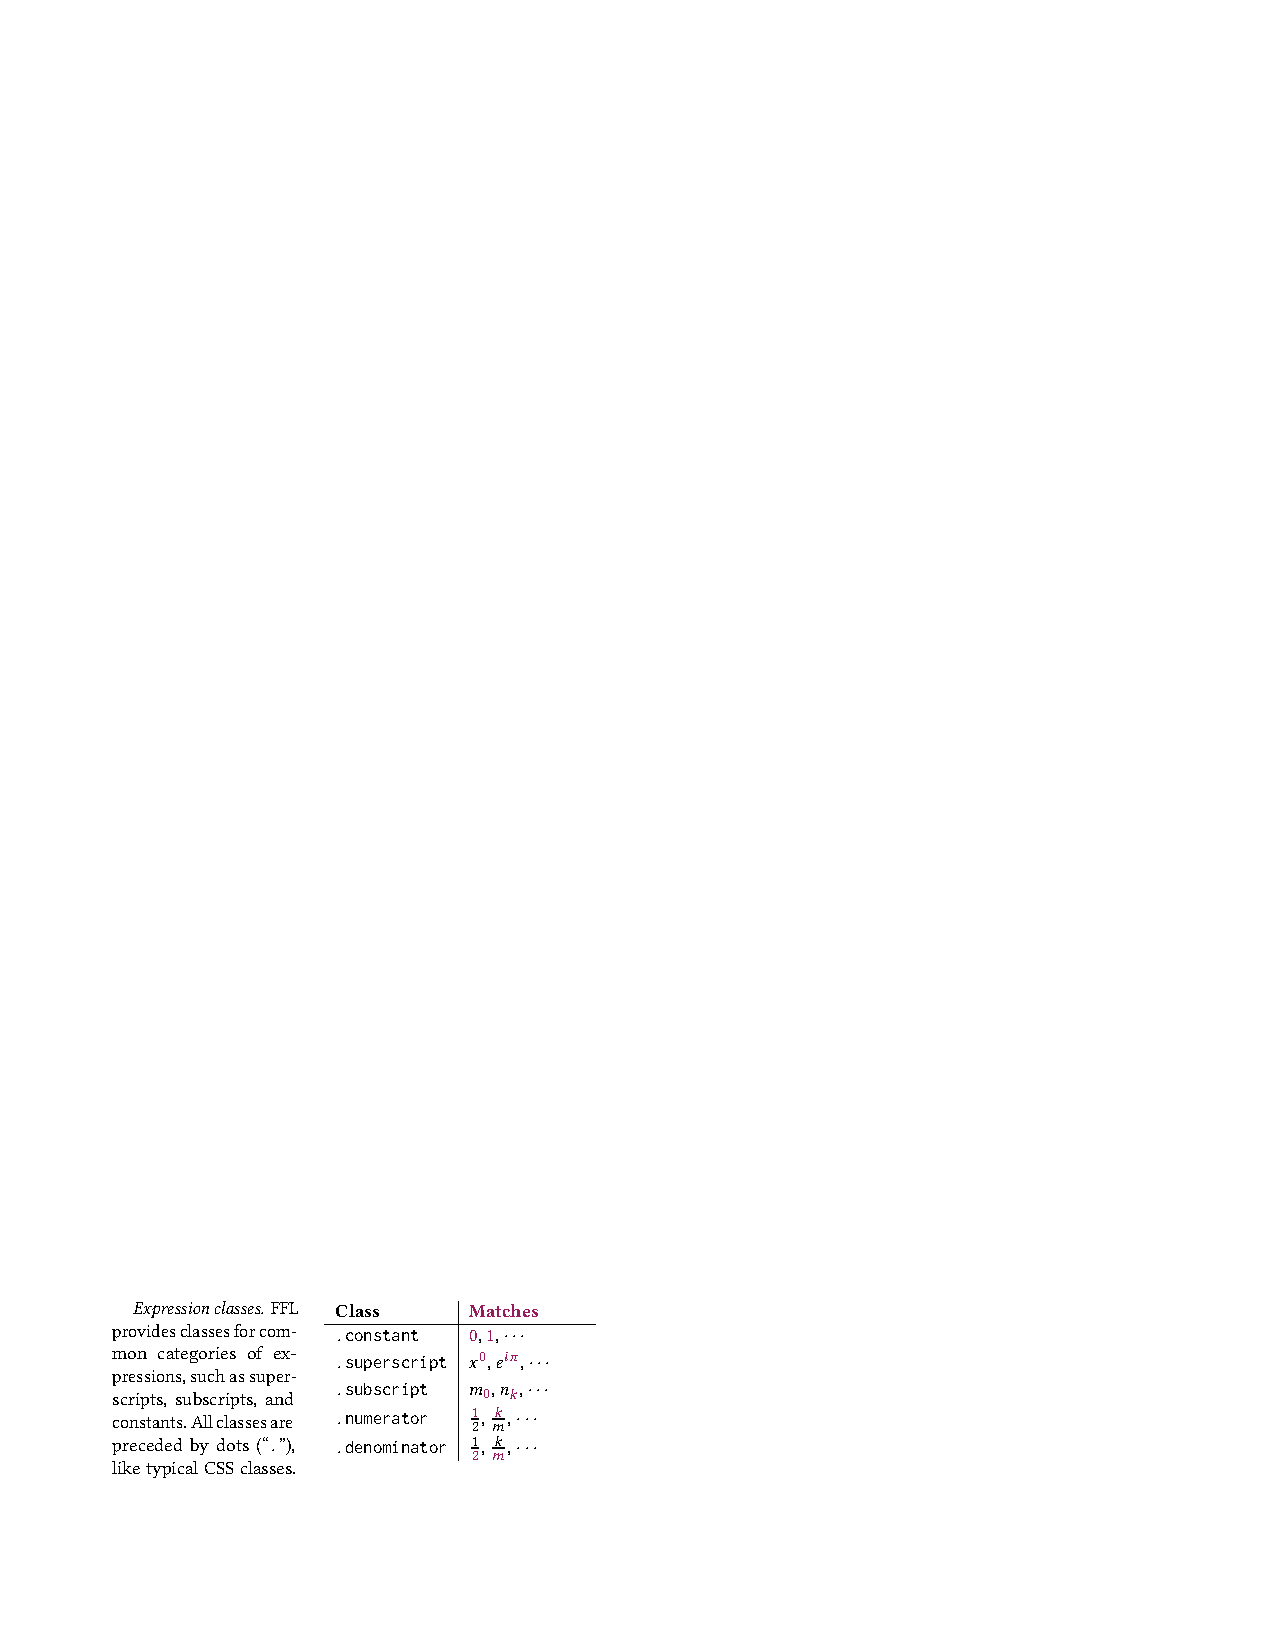
\includegraphics[width=1.02\linewidth]{fig/P6-1.pdf}} }{ \setlength{\columnsep}{1em}%
\begin{wrapfigure}[8]{r}{0.6\columnwidth}
% \begin{center}
    \vspace{-1.4em}
    \hspace{1ex}
    \begin{tabularx}{.54\columnwidth}{l|l}
    \textbf{Class}   & \textcolor{magenta}{\textbf{Matches}}                                 \\\hline
    \texttt{.constant}    & $\textcolor{magenta}{0}$, $\textcolor{magenta}{1}$, $\cdots$                     \\[2pt]
    \texttt{.superscript} & $x^{\textcolor{magenta}{0}}$, $e^{\textcolor{magenta}{i\pi}}$, $\cdots$          \\[2pt]
    \texttt{.subscript}   & $m_{\textcolor{magenta}{0}}$, $n_{\textcolor{magenta}{k}}$, $\cdots$             \\[2pt]
    \texttt{.numerator}   & $\frac{\textcolor{magenta}{1}}{2}$, $\frac{\textcolor{magenta}{k}}{m}$, $\cdots$ \\[2pt]
    \texttt{.denominator} & $\frac{1}{\textcolor{magenta}{2}}$, $\frac{k}{\textcolor{magenta}{m}}$, $\cdots$ \\
    \end{tabularx}
    \Description{A table of predefined classes, where each row shows the name of the class and examples of expressions the class matches. Every class name is preceded by a period. “dot-constant” matches numerical constants like 0 or 1. Superscripts, subscripts, numerator, and denominator match the mathematical structures of the same name.}
% \end{center}
\end{wrapfigure} } 


\paragraph{Expression classes} FFL provides classes for common categories of expressions, such as superscripts, subscripts, and constants. All classes are preceded by dots (``\texttt{.}''), like typical CSS classes. Supported classes are shown in the inset figure. These classes become particularly powerful when used within combinators, permitting an author to select, for instance, squares as the appearance of the literal ``\texttt{$2$}'' within superscripts.

% \paragraph{Pre-defined classes} For convenience, we also pre-configured
% a few commonly used categories of tokens. Note that these are all prefixed by a
% period (\texttt{.}) and we choose to call them ``classes'' to stay within the analogy to CSS. We currently have the classes below,
\paragraph{Indexed groups} To disambiguate between selections, we offer another special class named ``\texttt{.group}'', referring to portions of the formula markup surrounded by double braces (e.g. \texttt{\{\{}\dots\texttt{\}\}}). \zed{The modifier ``\texttt{:nth($i$}\texttt{)}'' can be appended to any selector to select the $i$-{th} matching expression. Authors select a specific group by using the modifier in conjunction with the ``\texttt{.group}'' selector. }

% \andrew{@Zed: scope selection features, including "nth" and indexed groups}

\paragraph{Combinators}
Selectors can be composed to make them more general or more precise. Selections can be made more precise with the intersection combinator, ``\texttt{{intersection}(}{\textit{selector1}, \textit{selector2}, \textit{...}}{\texttt{)}},'' which selects expressions matching all selectors provided as arguments. A shorthand for intersection is provided as ``\texttt{\textit{selector1} \textit{selector2} \textit{...}},'' which is reminiscent of CSS's compound selectors; with this shorthand authors can express intersections as if they were selecting \texttt{selector2} from within \texttt{selector1}. The union combinator, as with CSS, uses a comma (``\texttt{,}'') to separate selectors, matching any expression that matches one of the selectors.

% There are two ways of combining selectors. Using \texttt{{intersection}(}{\textit{selector1}, \textit{selector2}, \textit{...}}{\texttt{)}}, we select the intersection of the selections of all the selectors in the list, which also has the shorthand of optionally-space-separated selectors (i.e., \texttt{\textit{selector1} \textit{selector2} \textit{...}}). For example, \texttt{intersection(\$x\_?\$, .constant)} will only match constant subscript under $x$. Otherwise, comma-separated selectors on the top-level stands for the union of the selections. For example, \texttt{\$x\$, \$y\$} matches the entirety of $xyxxy$.

\paragraph{CSS Selectors} To select HTML elements from within an FFL style specification, an author can prepend an asterisk (``\texttt{*}'') to the name of a class (e.g., ``\texttt{*.cls0}'').

\subsubsection{Augmentations}

The FFL language supports specification of two kinds of augmentations: styles and labels. Permitted augmentations include color and labels, the two most commonly used kinds of augmentations according to a recent survey~\cite{ref:head2022math}.\footnote{An analysis of the spreadsheet in Head et al.'s~\cite{ref:head2022math} supplemental material shows 69\% of augmented formulas in their sample made use of either font color or labels.}
% Check or extend my work here: https://docs.google.com/spreadsheets/d/1YE7mw6Xrw6ebleQrfe13q2vv_0-J-Y1gPODhrhgwlrA/edit#gid=763614481

\paragraph{Style}
Styles are alterations to the expression elements, like color, font weight, and background. They correspond roughly to CSS properties, and share the same names (e.g., ``\texttt{color},'' ``\texttt{font-weight}''). Because these properties are transpiled into CSS, they accept all of the same property values as CSS (e.g., colors can be specified using HTML color codes, hex codes, ``\texttt{rgba(}\dots\texttt{)}'' values). As described in Section~\ref{sec:overlays}, some styles require additional processing on the backend to provide the expected styling behavior in the unique setting of HTML typeset math formulas.

% \subsubsection{Supported Style Properties}
% By implementing the selectors on top of web-technologies, we get some styling properties ``for free'' by using the identical CSS properties, such as \texttt{color} and \texttt{font-weight} which are among the most common style adjustments made to formulas. This also allows us some limited support for mixing in CSS stylings for non-math elements inside FFL styling by simpling adding any class selectors in the selector list, prefixed by an asterisk (\texttt{*}), in keeping with CSS convention for ``all elements,'' as it would be selecting elements external to math expressions, in contrast to the rest of \textit{FFL} styles. In the cases where default CSS behavior is not desired, among which we currently support \texttt{background-color}, where the CSS would be applied to each DOM element of the selected segment individually, we draw an additional under-/overlay in order to render the desired styles.

\paragraph{Labels}
FFL provides language primitives for creating and customizing labels that describe expressions. The ``\texttt{label}'' property allows an author to define and show a label for an expression: upon specifying this property, a label will appear next to the first appearance of that expression in a formula, connected to that expression with a leader line. The ``\texttt{label-marker}'' property allows the author to specify what kind of marker should connect the label to the expression. The marker can be either a \texttt{leader} line or an \texttt{extent} marker, i.e., a bracket shown in the margin; extent markers are particularly useful for labeling long expressions.

Label placement is automatic, and is designed to avoid overlapping labels and to place labels as close to their corresponding expressions as possible. \zed{A label is applied only once to any given formula; it is anchored to the first appearance of the labeled expression.} Should an author wish to customize the placement of labels, they may do so by defining the ``\texttt{label-position}'' property to place the label either ``\texttt{above}'' or ``\texttt{below}'' the formula.  To support further label customization, all labels allow values of ``\texttt{html(}\dots\texttt{)}'' (sanitized for security by default), or are generated as HTML text \texttt{span}s with the class ``\texttt{ffl-label}'' class. In this way, their appearance (e.g., font size, font family, color) can be configured with normal CSS properties by using the CSS selector ``\texttt{*.ffl-label}.''

% Another major feature feature we support in addition to CSS-enabled ones is labels, which is another common augmentation to math formulas \cite{ref:head2022math}. By default, using the \texttt{label} property draws a label with the property value as the label, along with a leader line drawn from the first group of selected elements, and a bracket marking the extent could be added using the property \texttt{label-marker: extent}. While the positioning of label text is mostly automatic, we also allow specifying whether a label should be above or below the formula through the property \texttt{label-position: above{\normalfont/}below}.

\subsection{Live runtime}

FFL was designed to be incorporated into arbitrary web-based text editing tools as a live styling utility, and for integration into articles generated from these editors. In this section, we describe how the runtime to support integration as a live styling tool.

% The vision of FFL is of a toolkit that can be incorporated into arbitrary web editing environments as a dependency (and in any web articles that are generated from them). The toolkit has been designed with a particular focus on supporting live application of styles and augmentations, to support rapid iteration.

\subsubsection{FFL library}
% \subsubsection{Core Library}

To ease the work involved in integration, FFL is implemented as a light wrapper around widely-used \textit{KaTeX}~\cite{tool:katex} tool. KaTeX is a tool that typesets LaTeX formulas on web pages. It is used in a variety of web-based authoring tools, including Dropbox Paper, Observable, Gatsby, Messenger, and Quill. \zed{It is also one of the supported formula rendering engines in Jupyter Lab~\cite{jupyterlab-katex}}.
% , and \zed{has gained official support as a lightweight alternative to MathJax in Jupyter Lab 

To integrate FFL into a web authoring environment, a developer would do the following. First, they would create editor widgets (like text areas) for authors to write FFL in. Second, they would replace calls to KaTeX's formula typesetter with a call to a nearly equivalent API on FFL. That method has the signature:

% \vspace{-.5ex}
\begin{Verbatim}
ffl.render(latex: string, ffl: string,
  renderTo: HTMLElement, options?: KatexOptions): void
\end{Verbatim}
% \vspace{-.5ex}
where ``\texttt{latex}'' is the LaTeX markup for the formula, the ``\texttt{ffl}'' parameter takes in the FFL style specification, ``\texttt{renderTo}'' is a reference to the HTML element into which to render the augmented formula, and ``\texttt{options}'' is an object of KaTeX options for typesetting the formula. If called without a ``\texttt{renderTo}'' target, the method returns the HTML string for the rendered formula.

% \andrew{The library's support for error-handling is currently limited to simply reporting if a syntax error was found, rather than indicating the source of the error. }

% The API of the core library closely mirrors that of \textit{KaTeX}\cite{tool:katex}, with the additional argument of \textit{FFL} styles, with the option to either render the formula to an HTML element or return an HTML string. The primary entry point resembles \texttt{ffl.render(latex: string, ffl: string, renderTo: HTMLElement, options?: KatexOptions): void}, while the option to render to an HTML string leaves out the \texttt{renderTo} argument, and instead returns the string. This library is purely programmatic can be used without a graphical interface and it handles single invocations of processing and rendering by interacting with \textit{KaTeX}. In order to preserve flexibility, we do not constrain the scope and frequency that the core library is invoked.

\subsubsection{Supporting live evaluation}\label{sec:live_evaluation}
To support live evaluation of an FFL style specification in an editing environment, the one necessity is to trigger a new call to ``\texttt{ffl.render}'' whenever the LaTeX or the FFL specification changes.
To demonstrate the feasibility of such an integration, we implemented a Markdown editing environment with live FFL integrated. To develop this environment, we first created a document editor as a simple text area. When authors write Markdown in the text area, the Markdown is passed to the \textit{markdown-it}~\cite{MarkdownIt} open source Markdown parser and then rendered into a document view next to the Markdown editor.

We created a pluggable \textit{markdown-it} extension to call the FFL API, rather than the KaTeX API, to render math formulas; the FFL API is called with an FFL style specification that authors write in another text box adjacent to the Markdown text box. Live evaluation is supported by triggering a parse of the Markdown when either the Markdown or the FFL specification is edited.  A demo of the authoring environment appears in the accompanying video. %% The speed of the runtime has been generally sufficient for the usability studies, although further testing is needed to validate its scalability to large math documents.

% \subsubsection{Accompanying Integrations} Primarily, we provide an example \textit{markdown-it}\cite{MarkdownIt} extension that allows {FFL} to be invoked to render math mode inside a markdown environment. In this case, it merely involves simple parsing rules for math blocks and rendering rules that invokes the core library accordingly. Similar integrations could conceivably be made with any other extensible document rendering engine built on web technologies.

% \subsubsection{Sample Editing Environment} With the \textit{markdown-it} integration, we build a simple editing environment with input for a single markdown document and a global set of \textit{FFL} style, along with live preview of said document, including the specified styles and augmentations. This is the main environment on which we base our lab study and observations.

% server rendering

% 3. The ability to add padding really easily in a familiar way (I think this doesn't work yet---merge with the next point.)
% 4. Additional affordances that CSS brings (changing font weight, adding background color, adding a border)

% We takes a slightly different approach yet again that is intended to fit into a different
% part of design space, revolving already popular platforms and tools with some considerations for simplicity.


% Based on these objectives, we make a few high-level foundational decisions:

% \subsection{Text-Based Typesetting}
% The first and the most fundamental is that most of our styles will be described
% by text input. One of the issues raised in \cite[Head et al.]{MAug} is that graphical
% interfaces often gets extremely visually busy and difficult to learn, in addition to
% that the support for reusing styles in a \textit{cross-cutting} fashion
% is generally fairly limited in most popular editing tools or require a lot of manual
% synchronization. Seeing as text-based typesetting tools has been generally more popular
% in more advanced and domain-specific editing tasks such as Markdown and LaTeX, along with
% the fact that LaTeX is already a common way to write math expressions, we have
% similarly chosen a textual/language-based approach.

% \subsection{Web-Native Implementation}
% We elected to build our system on top of \textit{KaTeX}, as Javascript-based library.
% This not only allows us relatively fast iteration turnaround time, as not only we have
% previous work using the similar technologies, but there are also ample open-source libraries
% and toolings for us to build upon and integrate\footnote{Figure \ref{md}} with.
% This way we are able to rely largely on existing infrastructure for supporting
% possible features.


% It also means that we are not constrained to a single editing environment,
% but rather new environments could be using any web-based technology,
% which has been an enduring and increasingly popular standard
% This way, any \textit{interactivity} can be easily achieved by building tools alongside such
% technologies, and given the variety of different environments that authors might use,
% we provide the opportunity to defer the choice to environment developers,
% and ultimately authors.

% \subsection{Familiar Syntax}
% Now, despite issues with graphical interfaces, we still need to be careful with the complexity
% of our language. While a complex language would likely allow us to be extremely expressive,
% we still aim for our tool to be relatively \textit{easy to use}. Especially when
% ``clucky syntax''\cite{MAug} is another concern with text-based tools, we intend to minimize
% the learning curve by mirroring chose mirror LaTeX as our syntax of choice for math expressions
% and CSS as our styling language, as both are commonly used and well supoorted
% for their respective purposes on the web. This not only simplifies implementation,
% but it is also our hope that it will create a relatively smooth learning curve
% for any user with experience in either or both. As writing them is already
% likely required to achieve similar effects in most current fashions, this experience
% should not be completely uncommon among authors who might find themselves needing
% styling of math expressions on the web.

% \subsection{Minimal API}
% Additionally, we restrict our API and responsibilities to processing the input and
% rendering only, mirroring again \textit{KaTeX}'s API so we could serve as
% a drop-in replacement. This should provide our API users\footnote{referring to developers
% who use our implementation to integrate \textit{FFL} with their own editing environments,
% in contrast to users of an authoring environment that might support \textit{FFL},
% which will be referred to more commonly as ``authors''} sufficient flexibility
% in the context of editing environments, minimizing the need for us to intervene to
% implement features for individual environments. For example,
% the possible \textit{interactivity} mentioned above becomes a simple matter of
% calling our API to re-render when the content of the document source has changed.
